%Title

%----------------------------------------------------------------------------------------
%	PACKAGES AND OTHER DOCUMENT CONFIGURATIONS
%----------------------------------------------------------------------------------------
\documentclass[letterpaper,12pt]{article}
%Graph
\usepackage{tabularx} % extra features for tabular environment
\usepackage{diagbox}
\usepackage[fleqn]{amsmath}  % improve math presentation
\usepackage{graphicx} % takes care of graphic including machinery
\usepackage{epstopdf}  
\usepackage[margin=1in,letterpaper]{geometry} % decreases margins
\usepackage{cite} % takes care of citations
\usepackage[final]{hyperref} % adds hyper links inside the generated pdf file
    \hypersetup{
	    colorlinks=true,       % false: boxed links; true: colored links
	    linkcolor=blue,        % color of internal links
	    citecolor=blue,        % color of links to bibliography
	    filecolor=magenta,     % color of file links
	    urlcolor=blue         
    }    
%Font
\usepackage{xeCJK,indentfirst}         %中文包&XeLaTex
    \setCJKmainfont[BoldFont=STZhongsong, ItalicFont=STKaiti]{STSong}
    \setCJKsansfont[BoldFont=STHeiti]{STXihei}
    \setCJKmonofont{STFangsong}
\usepackage{fontspec}
    \setmainfont{Times New Roman}
    \setsansfont{Arial}
%Picture
\usepackage{tikz}
    \usetikzlibrary{arrows}
\usepackage{asymptote}
\usepackage{algorithm}  
\usepackage{algpseudocode}  
\usepackage{amsmath}  
\renewcommand{\algorithmicrequire}{\textbf{Input:}}  % Use Input in the format of Algorithm  
\renewcommand{\algorithmicensure}{\textbf{Output:}} % Use Output in the format of Algorithm 
\usepackage{listings}
 \lstset{breaklines}




\begin{document}
%----------------------------------------------------------------------------------------
%	TITLE SECTION
%----------------------------------------------------------------------------------------
\title{Problem 1:Poisson Equation}
\author{Ruipeng Li, School of Physics, 1400011365}
\date{\today}
\maketitle

%----------------------------------------------------------------------------------------
%	ABSTRACT SECTION
%----------------------------------------------------------------------------------------
\begin{abstract}	

程序的具体说明请参见README.md文件,本报告主要是进行一些算法的分析以及结果的报告。首先我们给出问题的描述和分析,接着我们会分析具体的算法和表现、误差,最后我们会讨论下计算结果的物理意义。代码请参见https://github.com/Viciberty/CP.

\end{abstract}
%----------------------------------------------------------------------------------------
%	SOLUTION SECTION
%----------------------------------------------------------------------------------------

\begin{section}{Analysis}
    我们要求的是$Poisson$方程的电势场。主流的做法有两大类,第一类是先对一个维度做傅里叶变换,然后求解$ODE$,第二大类是直接采用格点空间法,常见的成熟做法有有限元方法、有限差分法。在本题中,我们采用的是格点空间法,利用中心差分,然后再用迭代方法对该方程组进行迭代求解。
	\begin{itemize}
		\item 先取网格,由边界条件,我们取柱坐标划分;
        \item 选取中心差分,用差分方程代替微分方程;
        \item 确认边界条件,采用电四极矩展开,并列出方程组;
		\item 利用超松弛迭代法对该方程组进行求解;
	\end{itemize}\par
	我们的目标是尽量提高计算的精度与速度(迭代方法还有收敛速度)。\par

    \subsection{列出柱坐标下微分方程}
    \begin{align*}
        \nabla^2\phi &= \frac{1}{\rho}\frac{\partial}{\partial{\rho}}(\rho\frac{\partial \phi}{\partial \rho})+\frac{\partial^2\phi}{\partial z^2}\\
        &= \frac{\partial^2 \phi}{\partial \rho^2} + \frac{1}{\rho}\frac{\partial \phi}{\partial \rho} + \frac{\partial^2\phi}{\partial z^2}\\
        &=  - \frac{0.8}{1+e^{(\sqrt{\rho^2+z^2}-10(1+1.0Y_2^0+0.5Y_3^0))/0.6}}\\
    \end{align*}
    where, $$Y_2^0(\rho,z)=\frac{1}{4}\sqrt{\frac{5}{\pi}}(\frac{3z^2}{\rho^2+z^2}-1)$$
    $$Y_3^0(\rho,z)=\frac{1}{4}\sqrt{\frac{7}{\pi}}(\frac{5z^3}{(\rho^2+z^2)^{1.5}}-\frac{3z}{\sqrt{\rho^2+z^2}})$$
        \indent 我们采用柱坐标划分,取$\{r_k\}\{z_k\}(k=0,1,2,\cdots,N)$ 分别代表$\rho$和$z$,对此均匀划分了N段。

    \subsection{利用中心差分方法求出导数}
        记$\phi _{i,j}$第一个下标代表r,第二个下标代表z.
        $$(\frac{\partial^2 \phi}{\partial r^2})_{i,j}=\frac{\phi_{i-1,j}+\phi_{i+1,j}-2\phi_{i,j}}{(\Delta r)^2}$$
        $$(\frac{\partial^2 \phi}{\partial z^2})_{i,j}=\frac{\phi_{i,j-1}+\phi_{i,j+1}-2\phi_{i,j}}{(\Delta z)^2}$$
        $$(\frac{1}{r}\frac{\partial \phi}{\partial r})_{i,j}=\frac{\phi_{i+1,j}-\phi_{i-1,j}}{2\Delta r r_i}$$
        化为线性方程组
        $$[\frac{1}{(\Delta r)^2}-\frac{1}{2(\Delta r) r_i}]\phi_{i-1,j}+[\frac{1}{(\Delta r)^2}+\frac{1}{2(\Delta r) r_i}]\phi_{i+1,j}+\frac{1}{(\Delta z)^2}\phi_{i,j-1}+\frac{1}{(\Delta z)^2}\phi_{i,j+1}$$
        $$= 2[\frac{1}{(\Delta z)^2}+\frac{1}{(\Delta r)^2}]\phi_{i,j}- \frac{0.8}{1+e^{(\sqrt{r_i^2+z_j^2}-10(1+1.0Y_2^0+0.5Y_3^0))/0.6}}$$
        我们将$\phi_{i,j}$排为$N_r \times N_Z$维向量,转为一维数组储存,$(i,j)->(i\times N_z+j)$, 接下来我们要求解这个稠密线性方程组$AX=b$,A为$(N_r*N_z)^2$维度。
        $$A_{i\times N_z+j,(i-1)\times N_z+j}=\frac{1}{(\Delta r)^2}-\frac{1}{2(\Delta r) r_i}$$
        $$A_{i\times N_z+j,(i+1)\times N_z+j}=\frac{1}{(\Delta r)^2}+\frac{1}{2(\Delta r) r_i}$$
        $$A_{i\times N_z+j,i\times N_z+j-1}=A_{i\times N_z+j,i\times N_z+j+1}=\frac{1}{(\Delta z)^2}$$

        $$A_{i\times N_z+j,i\times N_z+j}=-2[\frac{1}{(\Delta z)^2}+\frac{1}{(\Delta r)^2}]$$
        $$b_{i\times N_z+j}=- \frac{0.8}{1+e^{(\sqrt{r_i^2+z_j^2}-10(1+1.0Y_2^0+0.5Y_3^0))/0.6}}$$
        A的其余同行元素为0

    \subsection{确认边界条件}
        \subsubsection{$r=0$处边界条件}
            方程改写为:$$2\frac{\partial^2 \phi}{\partial r^2} + \frac{\partial^2\phi}{\partial z^2} = -f$$
            其中:
            $$(\frac{\partial^2 \phi}{\partial z^2})_{0,j}=\frac{\phi_{0,j-1}+\phi_{0,j+1}-2\phi_{0,j}}{(\Delta z)^2}$$

            $$(\frac{\partial^2 \phi}{\partial r^2})_{0,j}=\frac{2\phi_{1,j}-2\phi_{0,j}}{(\Delta r)^2}$$
            联立方程知道:
            $$\frac{1}{(\Delta z)^2}\phi_{0,j-1}+\frac{1}{(\Delta z)^2}\phi_{0,j+1}+\frac{4}{(\Delta r)^2}\phi_{1,j}=[\frac{4}{(\Delta r)^2}+\frac{2}{(\Delta z)^2}]\phi_{0,j}-f$$
            这样我们有
            $$A_{0\times N_z+j,0\times N_z+j-1}=\frac{1}{(\Delta z)^2}$$
            $$A_{0\times N_z+j,0\times N_z+j+1}=\frac{1}{(\Delta z)^2}$$
            $$A_{0\times N_z+j,1\times N_z+j}=\frac{4}{(\Delta r)^2}$$
            $$A_{0\times N_z+j,0\times N_z+j}=-[\frac{4}{(\Delta r)^2}+\frac{2}{(\Delta z)^2}]$$

        \subsubsection{$z=z_{max}$ 或 $z=z_{min}$ 或 $r=r_{max}$处边界条件}
            对于远场行为,我们可以有两种求法。第一种就是直接积分$\int \dfrac{\rho(r)}{r}dV$利用蒙卡均匀取点近似得到$E[\dfrac{\rho(r)}{r}]$或其他数值积分办法得到边界值,第二种就是利用电动力学里的电多极矩展开,展开到电四极矩。当然,我们也可以取特殊情况,即自然的边界条件,认为边界上的电势已经趋于0,来看看大致的形状。\par
            
            \indent \textbf{第一种方法}:计算二重积分$$\int_{D} \dfrac{\rho(\vec \xi)}{|\vec r-\vec \xi|}dV_\xi=\int_D\frac{\rho(\vec\xi)}{|\vec r-\vec \xi|}\xi_r d\xi_\varphi d\xi_rd\xi_z$$,我们简单取D为矩形,用计算机产生在D上均匀分布,且相互独立的随机变量的序列观测值$
        \{\xi_n\}$定义为$\{g(\xi_j)\};j=1,2,\cdots$是独立同分布随机序列,利用强大数律知道,
        $$\lim_{n \to \infty} \frac{1}{n} \sum\limits^{n}_{j=1} g(\xi_i)=E[g(\xi_1)]=\frac{1}{m(D)} \int_{D} g(x)dV,a.s.$$

            于是对于较大的n,
            $$\frac{m(D)}{n}\sum\limits^n_{j=1}g(\xi_i)\approx\int_{D}g(x)dx$$
            \indent 在本题中,我们需要计算如下积分,另D取三维$[0,r\_int\_Max]\times[0,2\pi]\times[z\_int\_Min,z\_int\_Max]$$$\frac{m(D)}{4\pi n}\sum\limits^n_{i=1}\frac{f(\vec\xi_i)}{|\vec\xi_i-\vec r|}\times (\xi_r)_i$$
            where
            $$m(D)=r\_int\_Max \times 2\pi \times (z\_int\_Max - z\_int\_Min) $$
            $$|\vec \xi_i-\vec r|=\sqrt{\xi_r^2+r^2-2r\xi_r cos\xi_\varphi + (\xi_z -z)^2}$$

            \indent \textbf{第二种方法}:计算电多极矩展开
            $$\varphi(\vec x)=\frac{1}{4\pi\epsilon_0}[\frac{Q}{R}-\vec p\cdot\nabla\frac{1}{R}+\frac{1}{6}\sum\limits_{i,j}D_{ij}\frac{\partial^2}{\partial x_i \partial x_j}\frac{1}{R}]+\cdots$$
            ,where
            $$Q=\int_V \rho(\vec x')dV'=\sum\limits_Vf(\rho,z)\Delta V=\sum\limits_V f(\rho,z)2\pi \rho \Delta\rho \Delta z,$$
            由对称性知系统只有沿z方向的电偶极矩
            $$\vec p=\int_V \rho(\vec x')\vec x'dV',p_z=\sum_Vf(\rho,z)z\Delta V=\sum_Vf(\rho,z)z\cdot 2\pi\rho\Delta \rho \Delta z $$
            由对称性知,系统有轴对称性,\textbf{D}仅有对角分量,且$D_{xx}=D_{yy}=-\frac{1}{2}D_{zz}$,只需计算$D_{zz}$
            $$D_{ij}=\int_V 3x_i'x_j'\rho(\vec x')dV',D_{zz}=\sum_V f(\rho,z)(3z^2-(\rho^2+z^2))\Delta V=\sum_V f(\rho,z)(2z^2-\rho^2)\cdot2\pi\rho\Delta\rho\Delta z$$
            这样,我们知道:
            $$\varphi^{(0)}=\frac{Q}{4\pi\epsilon_0R}$$
            $$\varphi^{(1)}=-\frac{1}{4\pi\epsilon_0}\vec p \cdot \nabla \frac{1}{R}=\frac{\vec p\cdot \vec R}{4\pi\epsilon_0 R^3}$$
            $$\varphi^{(2)}=\frac{1}{24\pi\epsilon_0}\sum\limits_{ij}D_{ij}\frac{\partial^2}{\partial x_i \partial x_j}\frac{1}{R}$$
            $$\varphi=\frac{1}{4\pi\epsilon_0}(\frac{Q}{\sqrt{\rho_0^2+z_0^2}}+\frac{\vec p\cdot \vec r}{(\rho_0^2+z_0^2)^{\frac{3}{2}}}+\frac{\textbf{D}:\vec e_r \vec e_r}{2(\rho_0^2+z_0^2)^{\frac{3}{2}}})$$
            $$\varphi=\frac{1}{4\pi\epsilon_0}(\frac{Q}{\sqrt{\rho_0^2+z_0^2}}+\frac{p_z z_0}{(\rho_0^2+z_0^2)^{\frac{3}{2}}}+\frac{D_{zz}(z_0^2-\frac{1}{2}\rho_0^2)}{2(\rho_0^2+z_0^2)^{\frac{5}{2}}})$$
            这样,我们通过计算电多极矩,带入如上的公式,就可以得到最后的$\varphi$。在编程时,我们需要做的就是积分得到电多极矩,在带入电势公式,求出边界上的电势值。但这里要注意电多极矩的展开条件$l <<r$,其中l为电荷尺度,r为电荷到要计算的场点的距离,本题中即边界值的电势。\\
            \indent 通过数值积分我们知道$$\frac{Q}{\epsilon_0}=4551.8,\frac{p_z}{\epsilon_0}=9528.8,\frac{D_{zz}}{\epsilon_0}=5.8513\times 10^5$$
            \indent 以上的结论是通过上次作业用蒙卡完成的数值积分,也经过了matlab的数值模拟验证,基本是一致的。\\

            \textbf{特殊情况}:\\ \indent 我们只要边界取得足够大,就可以做到让边界上的值趋于0。在这样的自然边界条件下,我们可以求得电势的分布,形状应该也是大致类似的。我们可以比较与以上两种情况的差别,从而看出边界条件对整个电势求解的影响。\\

            \indent 以上三种情况的精确程度取决于远场条件的满足情况,即我们取的边界的大小。在本题中,我们取了$$r\in[0,50]fm,z\in[-50,50]fm$$,这时电势已基本趋于0,也不至于运算量过大。

        \subsection{迭代求解线性方程组}
            这里我们讨论经典的迭代办法,而不考虑共轭梯度法,在柱坐标下,A并非一个对称正定的矩阵,故由共轭梯度法无法得到精确的解。\\
            \indent 程序中分别实现了雅克比迭代法和超松弛迭代法,由于矩阵规模太大,验证谱半径的难度比较大,故在此略去了验证收敛性和收敛速度的论证。通过经验性的尝试测试了下松弛系数,取了一个收敛速度较为优化的值。\\
            \\
            \textbf{雅克比迭代法}:\\
                这是比较经典的一种迭代算法,迭代法收敛的充要条件是迭代矩阵B的谱半径$\rho(\textbf{B})<1$. $\rho(\textbf{B})$越小,收敛速度越快。
                \begin{algorithm}[!htbp]  
                  \caption{Jacobi迭代法}  
                  \label{Jacobi迭代法}  
                  \begin{algorithmic}[1] 
                    \State \textbf{Do k=1,M}  
                    \State \quad $x_i:=(b_i-\sum\limits^n_{j=1,j\not =i}a_{ij}x_j^{(0)})/a_{ii}\quad (i=1,2,\cdots,n)$
                    \State \quad \textbf{if $(||x-x^{(0)}||<\epsilon)$ and $k\le$ M STOP}
                    \State \quad \textbf{if (k>M) STOP Not converged at given M and $\epsilon'$}
                    \State \quad $x_i^{(0)}:=x_i\quad (i=1,\cdots,n)$
                    \State \textbf{Enddo}
                  \end{algorithmic}  
                \end{algorithm}  
            \\
            \textbf{超松弛迭代法}:\\
                这是高斯-赛德尔法的推广,可以加快高斯-赛德尔的收敛速度。而其中的松弛系数$\omega$是一个在[1,2]的一个常数,一般通过经验来确定。
                \begin{algorithm}[!htbp]  
                  \caption{逐次超松弛迭代法(SOR)}  
                  \label{SOR迭代法}  
                  \begin{algorithmic}[1] 
                    \State \textbf{Do k=1,M}  
                    \State \quad $x_1:=(1-\omega)x_1^{(0)}+\omega(b_1-\sum\limits^n_{j=2}a_{1j}x_j^{(0)})/a_{11}$
                    \State \quad $x_i:=(1-\omega)x_i^{(0)}+\omega(b_i-\sum\limits^{i-1}_{j=1}a_{ij}x_j-\sum\limits^{n}_{j=i+1}a_{ij}x_j^{(0)})/a_{ii}\quad (i=2,...,n-1)$
                    \State \quad $x_n:=(1-\omega)x_n^{(0)}+\omega(b_n-\sum\limits^{n-1}_{j=1}a_{nj}x_j)/a_{nn}$
                    \State \quad \textbf{if $(||x-x^{(0)}||<\epsilon)$ and $k\le$ M STOP}
                    \State \quad \textbf{if (k>M) STOP Not converged at given M and $\epsilon'$}
                    \State \quad $x_i^{(0)}:=x_i\quad (i=1,\cdots,n)$
                    \State \textbf{Enddo}
                  \end{algorithmic}  
                \end{algorithm}  
\end{section}




\begin{section}{Results}
	\begin{subsection}{蒙卡计算的边界条件}
		首先,我们给出蒙卡计算的边界条件下计算出的柱坐标电势分布。(3325次迭代收敛,不超过1e-3)\textbf{可以看出,沿r轴方向,z=0处明显有一道沟!}\emph{一道沟!}\underline{一道沟!}
	 \begin{figure}[!htbp]
		\begin{center}
			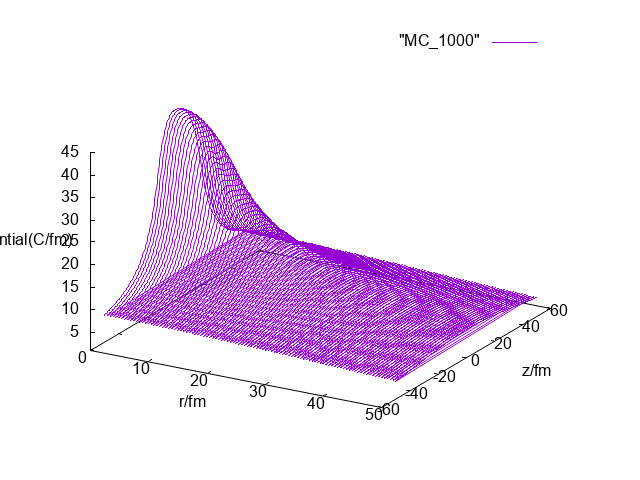
\includegraphics[scale=.6]{MC_1000.jpg}
		\end{center}
		\label{p1}
		\caption{蒙卡计算的边界条件下的电势分布}
	 \end{figure}
     \end{subsection}

     \begin{subsection}{电多极矩展开下的边界条件}
        接着,我们给出电多极矩展开下的边界条件下的电荷分布。(3325次迭代收敛,不超过1e-3)\textbf{可以看出,沿r轴方向,z=0处明显有一道沟!}\emph{一道沟!}\underline{一道沟!}
        \begin{figure}[!htbp]
        \begin{center}
            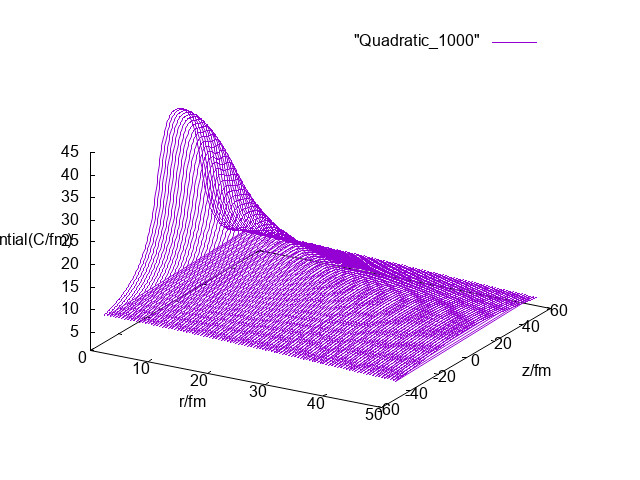
\includegraphics[scale=.6]{Quadratic_1000.jpg}
        \end{center}
        \label{p1}
        \caption{电多极矩展开下的边界条件}
     \end{figure}
     \end{subsection}

    \begin{subsection}{自然边界条件}
        接着,我们给出自然边界计算出的电势分布。(2551次迭代收敛,不超过1e-3)\textbf{可以看出,沿r轴方向,z=0处明显有一道沟!}\emph{一道沟!}\underline{一道沟!}
     \begin{figure}[!htbp]
        \begin{center}
            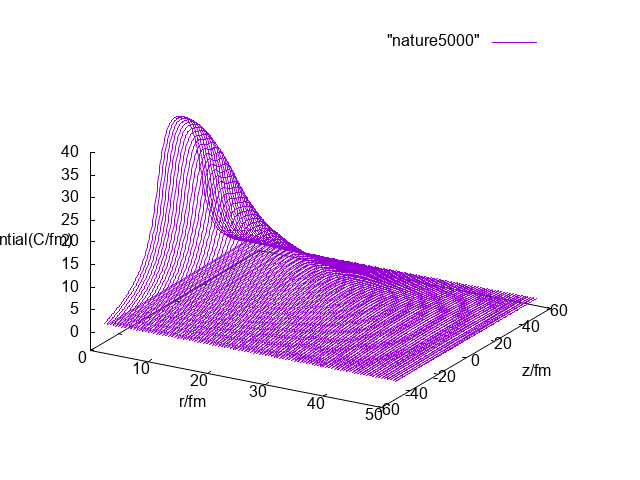
\includegraphics[scale=.6]{nature5000.jpg}
        \end{center}
        \label{p2}
        \caption{自然边界下的电势分布}
     \end{figure}
     \end{subsection}
     
     \begin{subsection}{分析}
     	我们对比分析了下三张图。可以看出在电多极矩展开算的边界条件下和蒙卡积分边界条件下,采用超松弛算法得到的最终电势几乎是一样的。而在边界取为0的时候,对电势的估计是有较大的误差的,边界的影响会相当大的影响峰值。同时也可以看出,大致形状也是基本类似的,符合我们的物理直觉。\\
     	\indent 同时采用超松弛的迭代算法,收敛速度还是可以的,在精度要求不高的前提下(取无穷范数为1e-3次方时),可以在3325步左右得到一个收敛的电势场分布。收敛性较jacobi方法稍微好些。\\
     	\indent \textbf{物理意义}:在这里我们求解了有源的静电学电势分布。这个源衰弱的特别快,我们取了一定的远场行为,求解了整个电场的分布情况。

     \end{subsection}
 \end{section}





\begin{section}{Appendix: Code}
\begin{lstlisting}
    //
//  main.cpp
//  PDE
//
//  Created by RP on 6/5/17.
//  Copyright © 2017 RP. All rights reserved.
//
using namespace std;
#include <iostream>
#include <math.h>
#include <cstdlib>
#include <ctime>
#define pi 3.1415926

#define N_r 100 //r_division
#define N_z 200 //z_division
#define r_Min 0  //r_min(fm)
#define r_Max 50 //r_max(fm)
#define z_Min -50 //z_min(fm)
#define z_Max 50 //z_max(fm)
#define epsilon 1e-20 //interval_epsilon

#define step 500 //steps
const double r_delta = r_Max*1.0/N_r;
const double z_delta = (z_Max-z_Min)*1.0/N_z;

const int r_point = N_r+1;
const int z_point = N_z+1;
double phi[r_point*z_point];
double phi_0[r_point*z_point];
double b_[r_point*z_point];
double A_[r_point*z_point][r_point*z_point];

int z_int_Min=0;
int z_int_Max=N_z;
int r_int_Min=0;
int r_int_Max=N_r;

/*****************************
 * Assistance Function
 *****************************/
double f(double r, double z)
{
    const double radius = sqrt(z*z+r*r);
    double cos = (radius==0)?0 : z / radius; //origin
    const double Y20 = 0.25*sqrt(5.0/pi)*(3*cos*cos-1);
    const double Y30 = 0.25*sqrt(7.0/pi)*(5*cos*cos*cos-3*cos);
    const double r0 = 10.0*(1+1.0*Y20+0.5*Y30);
    const double f_value = 0.8/(1+exp((radius-r0)/0.6));
    return f_value;
    }

double r(int i)
{
    if (i<r_point) {return r_Min+i*r_delta;}
    return -9999999999;
}

double z(int j)
{
    if (j<z_point){return z_Min+j*z_delta;}
    return -9999999999;
}

void print(double (*f)(double,double), double r_start=r_Min, double z_start=0, double r_n=r_point)
//print the value when z=z_start
{
    int i = 0 ;
    for (i=0;i<r_n;i++)
        cout << f(r_start+i*r_delta,z_start)<<endl;
    }


//Funtion
double MC(int i,int j);
double Quadratic(int i, int j);
double boundary(int i, int j, int method=1)
{
switch (method)
    {
    case 0:return MC(i,j);
    case 1:return Quadratic(i,j);
    case 2:return 0;
    default: return -999999999;
    }
}

double b(int x)
{
    int j = x % z_point;
    int i = x / z_point;
    if ((j==0) || (j==z_point-1) || (i==r_point-1) ) return boundary(i, j);
    return -f(r(i),z(j));
}

double A(int x, int y)
{
    int j = x % z_point;
    int i = x / z_point;
    //Inner Condition
    if ( (i>0) && (i<r_point-1) && (j>0) && (j<z_point-1))
    {
    if (y==(i-1)*z_point+j) {return 1/(r_delta*r_delta)-1/(2*r_delta*r(i));}
    if (y==(i+1)*z_point+j) {return 1/(r_delta*r_delta)+1/(2*r_delta*r(i));}
    if (y==i*z_point+j-1) {return  1/(z_delta*z_delta);}
    if (y==i*z_point+j+1) {return 1/(z_delta*z_delta);}
    if (y==i*z_point+j) {return -2*(1/(z_delta*z_delta)+1/(r_delta*r_delta));}
    }
    //r=0
    if ((i==0) && (j>0) && (j<z_point-1))
    {
        if (y==j-1) return 1.0/(z_delta*z_delta);
        if (y==j+1) return 1.0/(z_delta*z_delta);
        if (y==z_point+j) return 4.0/(r_delta*r_delta);
        if (y==j) return -(4.0/(r_delta*r_delta)+2.0/(z_delta*z_delta));
        }
    //Boundary Condition
    if ((j==0) || (j==z_point-1) || (i==r_point-1) )
        {
            if (y==i*z_point+j) return 1;
        }
    return 0;
    
}

/**************************************
 * Boundary Condition
 **************************************/

void interval()//Assume an interval for integrate
{
    
    int i= 0 ;
    for (i=1;i<z_point/2;i++){
        if ((b(i)>0?b(i):-b(i))< epsilon) z_int_Min = i;
    }
    for (i=z_point/2;i<z_point-1;i++){
        if ((b(i)>0?b(i):-b(i))> epsilon) z_int_Max = i+1;
    }
    for (i=z_point/2;i<(z_point-1)*r_point;i+=z_point){
        if ((b(i)>0?b(i):-b(i))> epsilon) r_int_Max = i/z_point+1;
    }
    cout<< z_int_Min<<" "<<z_int_Max<<" "<<r_int_Max<<endl;
    cout<<z(z_int_Min)<<" "<<z(z_int_Max)<< " "<<r(r_int_Max)<<endl;
}


double random(double start, double end)
{
    return start+(end-start)*rand()/(RAND_MAX );
}

double MC(int i,int j)//r(i),z(j) boudndary condition with MC
{
    const int N=1000000;
    double D = r(r_int_Max) * 2.0 * pi * (z(z_int_Max) - z(z_int_Min));
    int count;
    double sum=0;
    double xi_r,xi_z,xi_phi,distance;
    srand(unsigned(time(0)));
    for (count=0;count<N;count++)
    {
        xi_r = random(0,r(r_int_Max));
        xi_phi = random(0,2*pi);
        xi_z = random(z(z_int_Min),z(z_int_Max));
 //       cout<<xi_r<<" "<<xi_phi<<" "<<xi_z<<endl;
        distance = sqrt(xi_r*xi_r+r(i)*r(i)-2*r(i)*xi_r*cos(xi_phi)+(xi_z-z(j))*(xi_z-z(j)));
        sum+= f(xi_r,xi_z)*1.0/distance * xi_r;
        }
        return sum*1.0*D/N/4/pi;
    }

double Quadratic(int i,int j)//Multiple moment expansion
{
    double varphi_0,varphi_1,varphi_2;
    varphi_0 = 4551.8/sqrt(r(i)*r(i)+z(j)*z(j));
    varphi_1 = 9528.8*z(j)/(sqrt(r(i)*r(i)+z(j)*z(j))*sqrt(r(i)*r(i)+z(j)*z(j))*sqrt(r(i)*r(i)+z(j)*z(j)));
    varphi_2 = 585130*(z(j)*z(j)-0.5*r(i)*r(i))/(2*(sqrt(r(i)*r(i)+z(j)*z(j))*sqrt(r(i)*r(i)+z(j)*z(j))*sqrt(r(i)*r(i)+z(j)*z(j)))*(sqrt(r(i)*r(i)+z(j)*z(j))*sqrt(r(i)*r(i)+z(j)*z(j))*sqrt(r(i)*r(i)+z(j)*z(j)))*(sqrt(r(i)*r(i)+z(j)*z(j))*sqrt(r(i)*r(i)+z(j)*z(j))*sqrt(r(i)*r(i)+z(j)*z(j))));
    return (varphi_0+varphi_1+varphi_2)/(4*pi);
}
    
/**************************************
* Linear Equation Solution
**************************************/
double norm(int n=-1)//n-norm
{
    int count;
    double sum=0;
    for (count=0;count<z_point*r_point;count++)
    {
        sum = ((phi_0[count]-phi[count])*(phi_0[count]-phi[count])>sum)?(phi_0[count]-phi[count])*(phi_0[count]-phi[count]):sum;
    }
    return sqrt(sum);
}

double Jaccobi(int M, double e=1e-3)
{
    int count=0;
    int i,j=0;
    double sum=0;
    while (count<M)
    {
        for (i=0;i<r_point*z_point;i++){
            sum=0;
            for (j=0;j<r_point*z_point;j++)
            {
                if (i!=j) sum+=A_[i][j]*phi_0[j];
            }
            phi[i]=(b_[i]-sum)/A_[i][i];
        }
        if (norm(2)<e) {cout<<"success!"<<endl; break;}
        for (i=0;i<r_point*z_point;i++){
            phi_0[i] = phi[i];
        }
        count++;
    }
    return 0;
}

double SOR(int M, double omega=1.1, double e=1e-3)
{
    int count=0;
    int tmp,i,j=0;
    double sum=0,sum2=0;
    while (count<M)
    {
        for (i=0;i<r_point*z_point;i++){
            sum=sum2=0;
            if (i==0)
            {   for (j=1;j<r_point*z_point;j++) sum+=A_[i][j]*phi_0[j];
                phi[i]= (1-omega)*phi_0[i]+omega*(b_[i]-sum)/A_[i][i];
            }
            else if (i==r_point*z_point-1)
            {
                for (j=0;j<r_point*z_point-1;j++) sum+=A_[r_point*z_point-1][j]*phi[j];
                phi[i]= (1-omega)*phi_0[i]+omega*(b_[i]-sum)/A_[i][i];
            }
            else //其他
            {
                for (j=0;j<i;j++) sum+=A_[i][j]*phi[j];
                for (j=i+1;j<r_point*z_point;j++) sum2+=A_[i][j]*phi_0[j];
                phi[i]=(1-omega)*phi_0[i]+omega*(b_[i]-sum-sum2)/A_[i][i];
                
            }
            
        }

        if (norm(2)<e) {cout<<"success!"<<endl; break;}
        for (i=0;i<r_point*z_point;i++)
        {
            phi_0[i] = phi[i];
        }
        count++;
    }
    return 0;
 }

/**************************************
 * Main Procedure
 **************************************/

int main(int argc, const char * argv[]) {
    int i,j = 0 ;

//Initialization
    for (i=0;i<r_point*z_point;i++){
        phi[i]=0;
        phi_0[i]=0;
        b_[i]=b(i);
        for (j=0;j<r_point*z_point;j++) A_[i][j]=A(i,j);
    }
 

/*
//test linear equation solution!
    for (i=0;i<r_point*z_point;i++){
        phi[i]=0;
        phi_0[i]=0;
        b_[i]=0;
        for (j=0;j<r_point*z_point;j++) A_[i][j]=0;
    }
    b_[0]=b_[1]=0;
    b_[2]=b_[3]=1;
    A_[0][0]=A_[1][1]=A_[2][2]=A_[3][3]=4;
    A_[0][1]=A_[0][2]=A_[1][0]=A_[1][3]=A_[2][0]=A_[2][3]=A_[3][1]=A_[3][2]=-1;

*/

//    interval();
//    cout<<"r="<<r(0)<<" z="<<z(200)<<" "<<MC(1,200)<<endl;
//    for (i=0;i<r_point;i++)
//        cout<<b(i*z_point+1)<<endl;
    
//Execution and Output
 //   Jaccobi(step);
    SOR(step);

    for (i=0;i<r_point;i++) 
    {
        for (j=0;j<z_point;j++) cout<<r(i)<<" "<<z(j)<<" "<<phi[i*z_point+j]<<endl;
    }

    //    cout << "Hello, World!\n";
    return 0;
}

    \end{lstlisting}
  \end{section}

%----------------------------------------------------------------------------------------
%	CITATION SECTION
%----------------------------------------------------------------------------------------
%\bibliography{a}
%\bibliographystyle{IEEEtran}

\end{document}